% Created by tikzDevice version 0.6.2-92-0ad2792 on 2012-11-14 12:23:43
% !TEX encoding = UTF-8 Unicode
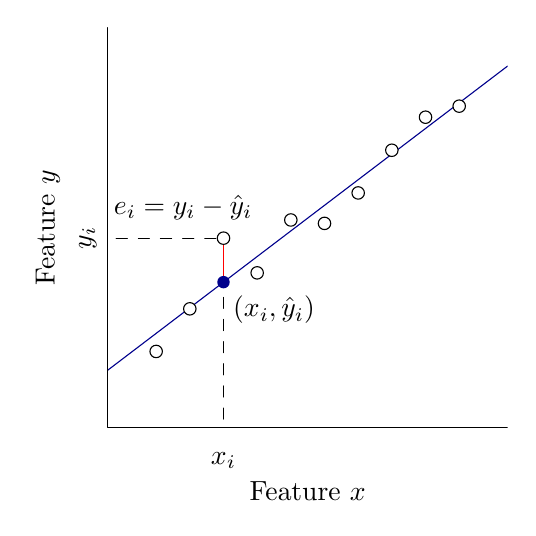
\begin{tikzpicture}[x=1pt,y=1pt]
\definecolor[named]{fillColor}{rgb}{1.00,1.00,1.00}
\path[use as bounding box,fill=fillColor,fill opacity=0.00] (0,0) rectangle (173.45,173.45);
\begin{scope}
\path[clip] (  0.00,  0.00) rectangle (173.45,173.45);
\definecolor[named]{drawColor}{rgb}{0.00,0.00,0.00}

\node[text=drawColor,anchor=base,inner sep=0pt, outer sep=0pt, scale=
  1.00] at (101.18,  2.51) {Feature $x$};

\node[text=drawColor,rotate= 90.00,anchor=base,inner sep=0pt, outer
  sep=0pt, scale=  1.00] at (  9.71,101.18) {Feature $y$};
\end{scope}
\begin{scope}
\path[clip] ( 28.91, 28.91) rectangle (173.45,173.45);
\definecolor[named]{drawColor}{rgb}{0.00,0.00,0.55}

\path[draw=drawColor,line width= 0.4pt,line join=round,line cap=round] ( 28.91, 49.66) -- (173.45,159.60);
\definecolor[named]{drawColor}{rgb}{0.00,0.00,0.00}

\path[draw=drawColor,line width= 0.4pt,dash pattern=on 4pt off 4pt ,line join=round,line cap=round] (  0.00, 97.39) --
	( 70.76, 97.39);

\path[draw=drawColor,line width= 0.4pt,dash pattern=on 4pt off 4pt ,line join=round,line cap=round] ( 70.76,  0.00) --
	( 70.76, 81.50);
\definecolor[named]{drawColor}{rgb}{1.00,0.00,0.00}

\path[draw=drawColor,line width= 0.4pt,line join=round,line cap=round] ( 70.76, 81.50) --
	( 70.76, 97.39);
\definecolor[named]{fillColor}{rgb}{0.00,0.00,0.55}

\path[fill=fillColor] ( 70.76, 81.50) circle (  2.25);
\definecolor[named]{drawColor}{rgb}{0.00,0.00,0.00}
\definecolor[named]{fillColor}{rgb}{1.00,1.00,1.00}

\path[draw=drawColor,line width= 0.4pt,line join=round,line cap=round,fill=fillColor] ( 46.43, 56.45) circle (  2.25);

\path[draw=drawColor,line width= 0.4pt,line join=round,line cap=round,fill=fillColor] ( 58.59, 71.85) circle (  2.25);

\path[draw=drawColor,line width= 0.4pt,line join=round,line cap=round,fill=fillColor] ( 70.76, 97.39) circle (  2.25);

\path[draw=drawColor,line width= 0.4pt,line join=round,line cap=round,fill=fillColor] ( 82.93, 84.85) circle (  2.25);

\path[draw=drawColor,line width= 0.4pt,line join=round,line cap=round,fill=fillColor] ( 95.09,103.96) circle (  2.25);

\path[draw=drawColor,line width= 0.4pt,line join=round,line cap=round,fill=fillColor] (107.26,102.73) circle (  2.25);

\path[draw=drawColor,line width= 0.4pt,line join=round,line cap=round,fill=fillColor] (119.43,113.73) circle (  2.25);

\path[draw=drawColor,line width= 0.4pt,line join=round,line cap=round,fill=fillColor] (131.59,129.16) circle (  2.25);

\path[draw=drawColor,line width= 0.4pt,line join=round,line cap=round,fill=fillColor] (143.76,141.10) circle (  2.25);

\path[draw=drawColor,line width= 0.4pt,line join=round,line cap=round,fill=fillColor] (155.93,145.09) circle (  2.25);

\node[text=drawColor,anchor=base,inner sep=0pt, outer sep=0pt, scale=  1.00] at ( 89.01, 68.94) {$(x_i, \hat{y}_i)$};

\node[text=drawColor,anchor=base,inner sep=0pt, outer sep=0pt, scale=  1.00] at ( 56.16,106.11) {$e_i = y_i - \hat{y}_i$};
\end{scope}
\begin{scope}
\path[clip] (  0.00,  0.00) rectangle (173.45,173.45);
\definecolor[named]{drawColor}{rgb}{0.00,0.00,0.00}

\node[text=drawColor,anchor=base,inner sep=0pt, outer sep=0pt, scale=  1.00] at ( 70.76, 15.71) {$x_i$};

\node[text=drawColor,rotate= 90.00,anchor=base,inner sep=0pt, outer sep=0pt, scale=  1.00] at ( 22.91, 97.39) {$y_i$};

\path[draw=drawColor,line width= 0.4pt,line join=round,line cap=round] ( 28.91,173.45) --
	( 28.91, 28.91) --
	(173.45, 28.91);
\end{scope}
\end{tikzpicture}
